\documentclass{standalone}
\usepackage{tikz}
\usetikzlibrary{patterns, positioning}

\begin{document}
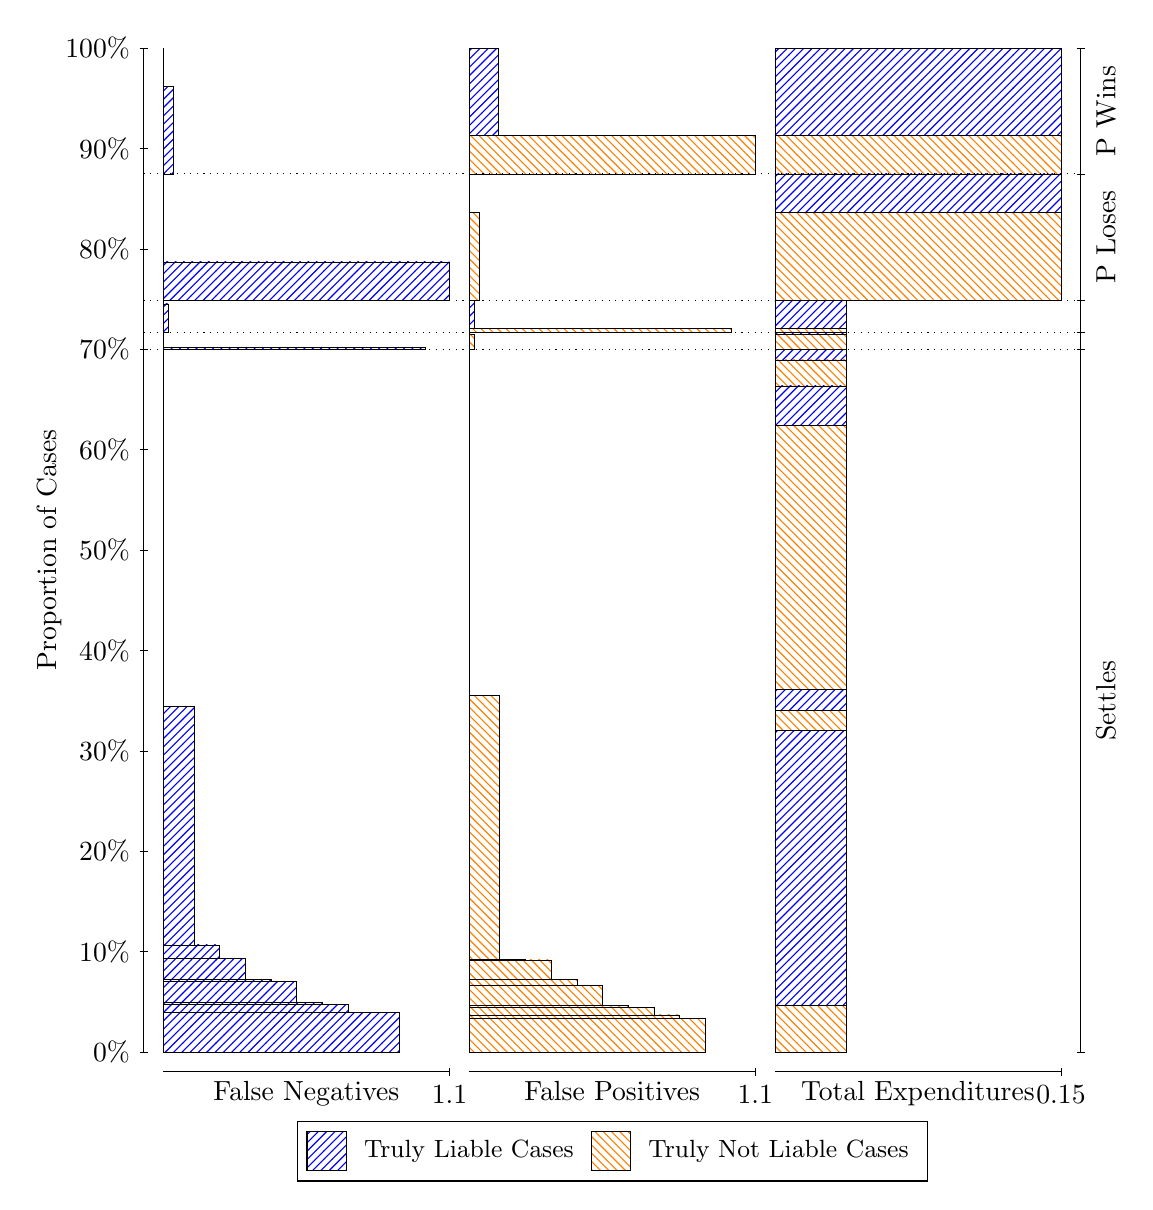
\begin{tikzpicture}
\draw[black, very thin] (1.5,1.75) -- (1.5,14.5);
\node[rotate=90, anchor=center] at (0.3, 8.125) {Proportion of Cases};
\draw[black, very thin] (1.45,1.75) -- (1.55,1.75);
\node[anchor=east] at (1.45, 1.75) {0\%};
\draw[black, very thin] (1.45,3.025) -- (1.55,3.025);
\node[anchor=east] at (1.45, 3.025) {10\%};
\draw[black, very thin] (1.45,4.3) -- (1.55,4.3);
\node[anchor=east] at (1.45, 4.3) {20\%};
\draw[black, very thin] (1.45,5.575) -- (1.55,5.575);
\node[anchor=east] at (1.45, 5.575) {30\%};
\draw[black, very thin] (1.45,6.85) -- (1.55,6.85);
\node[anchor=east] at (1.45, 6.85) {40\%};
\draw[black, very thin] (1.45,8.125) -- (1.55,8.125);
\node[anchor=east] at (1.45, 8.125) {50\%};
\draw[black, very thin] (1.45,9.4) -- (1.55,9.4);
\node[anchor=east] at (1.45, 9.4) {60\%};
\draw[black, very thin] (1.45,10.675) -- (1.55,10.675);
\node[anchor=east] at (1.45, 10.675) {70\%};
\draw[black, very thin] (1.45,11.95) -- (1.55,11.95);
\node[anchor=east] at (1.45, 11.95) {80\%};
\draw[black, very thin] (1.45,13.225) -- (1.55,13.225);
\node[anchor=east] at (1.45, 13.225) {90\%};
\draw[black, very thin] (1.45,14.5) -- (1.55,14.5);
\node[anchor=east] at (1.45, 14.5) {100\%};

\draw[black, very thin] (13.4,1.75) -- (13.4,14.5);
\draw[black, very thin] (13.35,1.75) -- (13.45,1.75);
\node[anchor=west] at (13.35, 1.75) {};
\draw[black, very thin] (13.35,10.674) -- (13.45,10.674);
\node[anchor=west] at (13.35, 10.674) {};
\draw[black, very thin] (13.35,10.888) -- (13.45,10.888);
\node[anchor=west] at (13.35, 10.888) {};
\draw[black, very thin] (13.35,11.299) -- (13.45,11.299);
\node[anchor=west] at (13.35, 11.299) {};
\draw[black, very thin] (13.35,12.901) -- (13.45,12.901);
\node[anchor=west] at (13.35, 12.901) {};
\draw[black, very thin] (13.35,14.5) -- (13.45,14.5);
\node[anchor=west] at (13.35, 14.5) {};

\draw[black, very thin, pattern color=blue, pattern=north east lines] (1.75,1.75) rectangle (4.7506,2.25);
\draw[black, very thin, pattern color=blue, pattern=north east lines] (1.75,2.25) rectangle (4.424,2.2572);
\draw[black, very thin, pattern color=blue, pattern=north east lines] (1.75,2.2572) rectangle (4.0974,2.3529);
\draw[black, very thin, pattern color=blue, pattern=north east lines] (1.75,2.3529) rectangle (3.7708,2.3829);
\draw[black, very thin, pattern color=blue, pattern=north east lines] (1.75,2.3829) rectangle (3.7708,2.3838);
\draw[black, very thin, pattern color=blue, pattern=north east lines] (1.75,2.3838) rectangle (3.4442,2.6496);
\draw[black, very thin, pattern color=blue, pattern=north east lines] (1.75,2.6496) rectangle (3.1176,2.6743);
\draw[black, very thin, pattern color=blue, pattern=north east lines] (1.75,2.6743) rectangle (2.791,2.9384);
\draw[black, very thin, pattern color=blue, pattern=north east lines] (1.75,2.9384) rectangle (2.4644,3.1101);
\draw[black, very thin, pattern color=blue, pattern=north east lines] (1.75,3.1101) rectangle (2.1378,6.1436);
\draw[black, very thin, pattern color=orange, pattern=north west lines] (1.75,6.1436) rectangle (1.75,10.674);
\draw[black, very thin, pattern color=blue, pattern=north east lines] (1.75,10.674) rectangle (5.0772,10.694);
\draw[black, very thin, pattern color=orange, pattern=north west lines] (1.75,10.694) rectangle (1.75,10.888);
\draw[black, very thin, pattern color=blue, pattern=north east lines] (1.75,10.888) rectangle (1.8112,11.251);
\draw[black, very thin, pattern color=orange, pattern=north west lines] (1.75,11.251) rectangle (1.75,11.299);
\draw[black, very thin, pattern color=blue, pattern=north east lines] (1.75,11.299) rectangle (5.3833,11.784);
\draw[black, very thin, pattern color=orange, pattern=north west lines] (1.75,11.784) rectangle (1.75,12.901);
\draw[black, very thin, pattern color=blue, pattern=north east lines] (1.75,12.901) rectangle (1.8725,14.015);
\draw[black, very thin, pattern color=orange, pattern=north west lines] (1.75,14.015) rectangle (1.75,14.5);
\draw[black, very thin, pattern color=orange, pattern=north west lines] (5.6333,1.75) rectangle (8.6339,2.1798);
\draw[black, very thin, pattern color=orange, pattern=north west lines] (5.6333,2.1798) rectangle (8.3073,2.2203);
\draw[black, very thin, pattern color=orange, pattern=north west lines] (5.6333,2.2203) rectangle (7.9807,2.3173);
\draw[black, very thin, pattern color=orange, pattern=north west lines] (5.6333,2.3173) rectangle (7.6541,2.3372);
\draw[black, very thin, pattern color=orange, pattern=north west lines] (5.6333,2.3372) rectangle (7.3275,2.5966);
\draw[black, very thin, pattern color=orange, pattern=north west lines] (5.6333,2.5966) rectangle (7.0009,2.6009);
\draw[black, very thin, pattern color=orange, pattern=north west lines] (5.6333,2.6009) rectangle (7.0009,2.6682);
\draw[black, very thin, pattern color=orange, pattern=north west lines] (5.6333,2.6682) rectangle (6.6743,2.9206);
\draw[black, very thin, pattern color=orange, pattern=north west lines] (5.6333,2.9206) rectangle (6.3478,2.9277);
\draw[black, very thin, pattern color=orange, pattern=north west lines] (5.6333,2.9277) rectangle (6.0212,6.2806);
\draw[black, very thin, pattern color=blue, pattern=north east lines] (5.6333,6.2806) rectangle (5.6333,10.674);
\draw[black, very thin, pattern color=orange, pattern=north west lines] (5.6333,10.674) rectangle (5.6946,10.869);
\draw[black, very thin, pattern color=blue, pattern=north east lines] (5.6333,10.869) rectangle (5.6333,10.888);
\draw[black, very thin, pattern color=orange, pattern=north west lines] (5.6333,10.888) rectangle (8.9605,10.936);
\draw[black, very thin, pattern color=blue, pattern=north east lines] (5.6333,10.936) rectangle (5.6946,11.299);
\draw[black, very thin, pattern color=orange, pattern=north west lines] (5.6333,11.299) rectangle (5.7558,12.416);
\draw[black, very thin, pattern color=blue, pattern=north east lines] (5.6333,12.416) rectangle (5.6333,12.901);
\draw[black, very thin, pattern color=orange, pattern=north west lines] (5.6333,12.901) rectangle (9.2667,13.386);
\draw[black, very thin, pattern color=blue, pattern=north east lines] (5.6333,13.386) rectangle (6.0007,14.5);
\draw[black, very thin, pattern color=orange, pattern=north west lines] (9.5167,1.75) rectangle (10.425,2.3372);
\draw[black, very thin, pattern color=blue, pattern=north east lines] (9.5167,2.3372) rectangle (10.425,5.8311);
\draw[black, very thin, pattern color=orange, pattern=north west lines] (9.5167,5.8311) rectangle (10.425,6.0906);
\draw[black, very thin, pattern color=blue, pattern=north east lines] (9.5167,6.0906) rectangle (10.425,6.3564);
\draw[black, very thin, pattern color=orange, pattern=north west lines] (9.5167,6.3564) rectangle (10.425,9.7094);
\draw[black, very thin, pattern color=blue, pattern=north east lines] (9.5167,9.7094) rectangle (10.425,10.209);
\draw[black, very thin, pattern color=orange, pattern=north west lines] (9.5167,10.209) rectangle (10.425,10.54);
\draw[black, very thin, pattern color=blue, pattern=north east lines] (9.5167,10.54) rectangle (10.425,10.674);
\draw[black, very thin, pattern color=orange, pattern=north west lines] (9.5167,10.674) rectangle (10.425,10.869);
\draw[black, very thin, pattern color=blue, pattern=north east lines] (9.5167,10.869) rectangle (10.425,10.888);
\draw[black, very thin, pattern color=orange, pattern=north west lines] (9.5167,10.888) rectangle (10.425,10.936);
\draw[black, very thin, pattern color=blue, pattern=north east lines] (9.5167,10.936) rectangle (10.425,11.299);
\draw[black, very thin, pattern color=orange, pattern=north west lines] (9.5167,11.299) rectangle (13.15,12.416);
\draw[black, very thin, pattern color=blue, pattern=north east lines] (9.5167,12.416) rectangle (13.15,12.901);
\draw[black, very thin, pattern color=orange, pattern=north west lines] (9.5167,12.901) rectangle (13.15,13.386);
\draw[black, very thin, pattern color=blue, pattern=north east lines] (9.5167,13.386) rectangle (13.15,14.5);
\draw[black, dotted] (1.5,10.674) -- (13.4,10.674);
\draw[black, dotted] (1.5,10.888) -- (13.4,10.888);
\draw[black, dotted] (1.5,11.299) -- (13.4,11.299);
\draw[black, dotted] (1.5,12.901) -- (13.4,12.901);
\draw[black, very thin] (1.75,1.5) -- (5.3833,1.5);
\node[anchor=north] at (3.5667, 1.5) {False Negatives};
\draw[black, very thin] (5.3833,1.45) -- (5.3833,1.55);
\node[anchor=north] at (5.3833, 1.45) {1.1};

\draw[black, very thin] (5.6333,1.5) -- (9.2667,1.5);
\node[anchor=north] at (7.45, 1.5) {False Positives};
\draw[black, very thin] (9.2667,1.45) -- (9.2667,1.55);
\node[anchor=north] at (9.2667, 1.45) {1.1};

\draw[black, very thin] (9.5167,1.5) -- (13.15,1.5);
\node[anchor=north] at (11.333, 1.5) {Total Expenditures};
\draw[black, very thin] (13.15,1.45) -- (13.15,1.55);
\node[anchor=north] at (13.15, 1.45) {0.15};

\node[black, centered, rotate=90] at (13.72, 6.2121) {Settles};


\node[black, centered, rotate=90] at (13.72, 12.1) {P Loses};
\node[black, centered, rotate=90] at (13.72, 13.7) {P Wins};

\draw (7.449999999999999,1.5) node[draw=none] (baseCoordinate) {};
\begin{scope}[align=center]
        \matrix[scale=0.5, draw=black, below=0.5cm of baseCoordinate, nodes={draw}, column sep=0.1cm]{
            \node[rectangle, draw, minimum width=0.5cm, minimum height=0.5cm, pattern=north east lines, pattern color=blue] {}; &
            \node[draw=none, font=\small] (B) {Truly Liable Cases}; &
            \node[rectangle, draw, minimum width=0.5cm, minimum height=0.5cm, pattern=north west lines, pattern color=orange] {}; &
            \node[draw=none, font=\small] (B) {Truly Not Liable Cases}; \\
            };
\end{scope}

\end{tikzpicture}
\end{document}